
\chapter{Hidden Markov Models}

In what follows our goal is to model \textbf{time series data}. This kind of data are observed from a process evolving in time, typically at different time steps $x_1, x_2, \dots, x_N$ (i.e. assuming a discrete model of time). Since sequential data often arise through measurement of time series, there is correlation between observations at different time steps. 

These data can come from very different domains: financial data, weather forecast data, speech data, epidemiological data. 

Markov Chains are natural models for sequential data, the following is a Markov Chain of order 1:
\vspace{0.5cm}
\begin{center}
    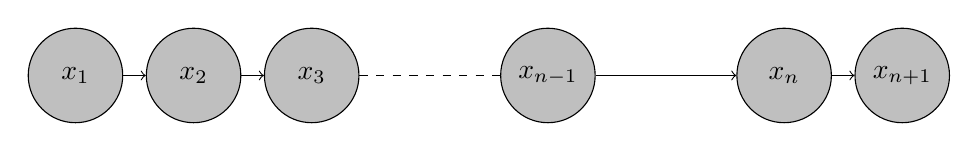
\begin{tikzpicture}
        % Nodes
        \node (x1) [circle, draw, fill=gray!50, minimum size=1.2cm] at (-4.5, 0) {\(x_1\)};
        \node (x2) [circle, draw, fill=gray!50, minimum size=1.2cm] at (-3, 0) {\(x_2\)};
        \node (x3) [circle, draw, fill=gray!50, minimum size=1.2cm] at (-1.5, 0) {\(x_3\)};
        \node (xn-1) [circle, draw, fill=gray!50, minimum size=1.2cm] at (1.5, 0) {\(x_{n-1}\)};
        \node (xn) [circle, draw, fill=gray!50, minimum size=1.2cm] at (4.5, 0) {\(x_n\)};
        \node (xn+1) [circle, draw, fill=gray!50, minimum size=1.2cm] at (6, 0) {\(x_{n+1}\)};
        
        % Edges
        \draw[->] (x1) -- (x2);
        \draw[->] (x2) -- (x3);
        \draw[dashed] (x3) -- (xn-1);
        \draw[->] (xn-1) -- (xn);
        \draw[->] (xn) -- (xn+1);
    
    \end{tikzpicture}
\end{center}
\vspace{0.5cm}
Since all he points (up to a certain step N) are observed, the factorization by the model is:
$$
p(x_1, x_2, \dots, x_N) = p(x_1) p(x_2 | x_1) p(x_3 | x_2) \dots p(x_N | x_{N-1})
$$

It holds that future observations are independent of all but the most recent observation:
$$
x_{n+1} \perp\!\!\!\perp x_1, x_2, \dots, x_n | x_n
$$

A \textbf{time homogeneus} process is a process whose transition probability does not change in time, i.e. such that $p(x_1|x_{n-q}) = p(x_2|x_1)$.

These chains are not always the best model for describing sequential observations, indeed often there is a deeper dependency on the past, and first-order Markov chains suffer from too short memory. 

In these cases, we can mode to \textbf{Markov models of order k}, where the dependency of $x_n$ is on the previous $k$ steps. The following is a second order Markov Chain:
\vspace{0.5cm}
\begin{center}
    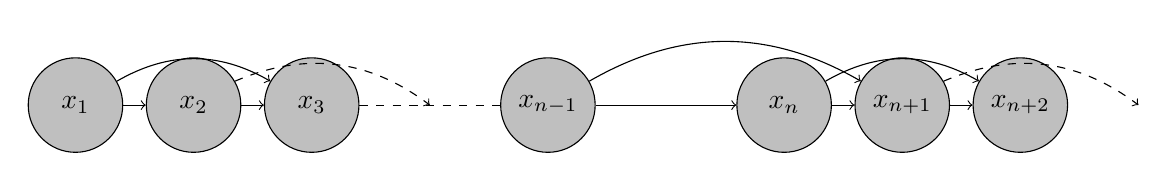
\begin{tikzpicture}
        % Nodes
        \node (x1) [circle, draw, fill=gray!50, minimum size=1.2cm] at (-4.5, 0) {\(x_1\)};
        \node (x2) [circle, draw, fill=gray!50, minimum size=1.2cm] at (-3, 0) {\(x_2\)};
        \node (x3) [circle, draw, fill=gray!50, minimum size=1.2cm] at (-1.5, 0) {\(x_3\)};
        \node (xn-1) [circle, draw, fill=gray!50, minimum size=1.2cm] at (1.5, 0) {\(x_{n-1}\)};
        \node (xn) [circle, draw, fill=gray!50, minimum size=1.2cm] at (4.5, 0) {\(x_n\)};
        \node (xn+1) [circle, draw, fill=gray!50, minimum size=1.2cm] at (6, 0) {\(x_{n+1}\)};
        \node (xn+2) [circle, draw, fill=gray!50, minimum size=1.2cm] at (7.5, 0) {\(x_{n+2}\)};

        % Edges
        \draw[->] (x1) -- (x2);
        \draw[->] (x2) -- (x3);
        \draw[->, bend left] (x1) to (x3);  % Curved line from x1 to x3
        \draw[->, bend left, dashed] (x2) to (0,0);  % Curved dashed line from x2 to xn-1
        \draw[->, bend left] (xn-1) to (xn+1);  % Curved line from xn-1 to xn+1
        \draw[->, bend left] (xn) to (xn+2);  % Curved line from xn to xn+2
        \draw[->, bend left, dashed] (xn+1) to (9, 0);
        \draw[dashed] (x3) -- (xn-1);
        \draw[->] (xn-1) -- (xn);
        \draw[->] (xn) -- (xn+1);
        \draw[->] (xn+1) -- (xn+2);
    \end{tikzpicture}
\end{center}

In this case, the factorization of the model is:
$$
p(x_1, x_2, \dots, x_N) = p(x_1)p(x_2|x_1)p(x_3|x_2,x_1) \dots p(x_{n+1}|x_n, x_{n-1}) \dots
$$

And it holds that:
$$
x_{n+2} \perp\!\!\!\perp x_{n-1} | x_n, x_{n+1}
$$

\textbf{Remark}: if $x_i$ are discrete, we talk about \textit{Markov chains}; if $x_i$ are continuous and $p(x_n|\dots)$ are Gaussian, we talk about \textit{autoregressive models} (of order k).

If we want to build a model for sequential data that is not limited to the Markov assumption of any order, we can rely on \textbf{state space models}, which introduce \textbf{latent variables}. In terms of graphical model, we have that latent variables from a Markov chain, and each of them corresponds to an observation:

\begin{center}
    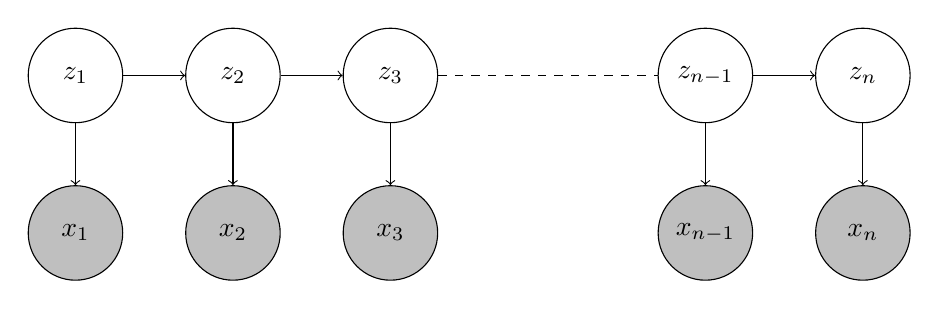
\begin{tikzpicture}
        % Nodes
        \node (x1) [circle, draw, fill=gray!50, minimum size=1.2cm] at (-4, 0) {\(x_1\)};
        \node (x2) [circle, draw, fill=gray!50, minimum size=1.2cm] at (-2, 0) {\(x_2\)};
        \node (x3) [circle, draw, fill=gray!50, minimum size=1.2cm] at (0, 0) {\(x_3\)};
        \node (xn-1) [circle, draw, fill=gray!50, minimum size=1.2cm] at (4, 0) {\(x_{n-1}\)};
        \node (xn) [circle, draw, fill=gray!50, minimum size=1.2cm] at (6, 0) {\(x_n\)};
        \node(z1) [circle, draw, minimum size=1.2cm] at (-4, 2) {\(z_1\)};
        \node(z2) [circle, draw, minimum size=1.2cm] at (-2, 2) {\(z_2\)};
        \node(z3) [circle, draw, minimum size=1.2cm] at (0, 2) {\(z_3\)};
        \node(zn-1) [circle, draw, minimum size=1.2cm] at (4, 2) {\(z_{n-1}\)};
        \node(zn) [circle, draw, minimum size=1.2cm] at (6, 2) {\(z_n\)};

        % Edges
        \draw[->] (z1) -- (x1);
        \draw[->] (z2) -- (x2);
        \draw[->] (z3) -- (x3);
        \draw[->] (zn-1) -- (xn-1);
        \draw[->] (zn) -- (xn);
        \draw[->] (z1) -- (z2);
        \draw[->] (z2) -- (z3);
        \draw[dashed] (z3) -- (zn-1);
        \draw[->] (zn-1) -- (zn);
    \end{tikzpicture}
\end{center}

If we consider two observations $x_i, x_j$, then $x_i \not\perp\!\!\!\perp x_j|\underbar{x}$ (with $\underbar{x} = x_1, \dots, x_n$) since there is not any obserbed node in the path from $x_i$ to $x_j$.

In order to describe the space models like the one above, we need:
\begin{itemize}
    \item \textbf{transition probabilities} $p(z_n|z_{n-1})$, which describe the evolution of the latent variables. They can be arranged in a matrix A s.t. $A_{ij} = p(z_n = j|z_{n-1} = i)$;
    \item \textbf{initial distribution} $p(z_1)$, specified by a vector $\pi$ s.t. $\pi_i = p(z_1 = i)$,
    \item \textbf{emission probabilities} $p(x_n|z_n)$, parametrized by $\psi$. The emission probability for discrete $x$ is a categorical distribution, for continuous $x$ is typically a Gaussian or a mixture of Gaussians.
\end{itemize}

\begin{definitionblock}[Hidden Markov Model]
    The \textbf{Hidden Markov Model} is a specific instance of the state space model described before, in which the latent variables $z_i$ are discrete. If instead the variables $z_i$ are continuous and the transition probabilities $p(z_i|z_{i-1})$ are Gaussian, we talk about \textbf{Linear Dynamical System}.
\end{definitionblock}

Consider the parameters $\Theta = (A, \pi, \psi)$ and the variables 
$$
\underbar{x}, \underbar{z} = (x_1, \dots, x_n, z_1, \dots, z_n)
$$
then 
$$
p(\underbar{x}, \underbar{z}|\Theta) = p(z_1|\pi) \left[ \prod_{n=2}^{N}p(z_n|z_{n-1}, A) \right] \left[\prod_{n=1}^{N}p(x_n|z_n, \psi)\right]
$$

\begin{exampleblock}
    We can graphically represent the states of $\underbar{z}$ and the transition matrix as follows (note that this is not a PGM):
    \begin{center}
        \begin{tikzpicture}
            % Nodes
            \node[draw, minimum size=1cm] (a) at (0,2) {a};
            \node[draw, minimum size=1cm] (b) at (-2,0) {b};
            \node[draw, minimum size=1cm] (c) at (2,0) {c};
        
            % Arrows
            \draw[->] (a) to [bend left] node[above] {$A_{ac}$} (c);
            \draw[->] (c) to [bend left] node[below] {$A_{cb}$} (b);
            \draw[->] (b) to [bend left] node[left] {$A_{ba}$} (a);
        
            % Self-loops
            \draw[->] (a) to[out=60,in=120,looseness=8] node[above] {$A_{aa}$} (a);
            \draw[->] (b) to [out=-135,in=135,looseness=8] node[left] {$A_{bb}$} (b);
            \draw[->] (c) to [out=-45,in=45,looseness=8] node[right] {$A_{cc}$} (c);
        

        \end{tikzpicture}
    \end{center}

    If we unfold the above graph over time, we obtain a sort of trellis diagram of the latent states:
    \begin{center}
        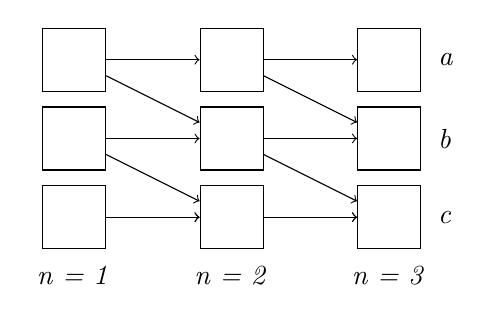
\begin{tikzpicture}
            % Nodes (grid layout)
            \node[draw, minimum size=0.8cm] (a1) at (0,2) {};
            \node[draw, minimum size=0.8cm] (b1) at (0,1) {};
            \node[draw, minimum size=0.8cm] (c1) at (0,0) {};
        
            \node[draw, minimum size=0.8cm] (a2) at (2,2) {};
            \node[draw, minimum size=0.8cm] (b2) at (2,1) {};
            \node[draw, minimum size=0.8cm] (c2) at (2,0) {};
        
            \node[draw, minimum size=0.8cm] (a3) at (4,2) {};
            \node[draw, minimum size=0.8cm] (b3) at (4,1) {};
            \node[draw, minimum size=0.8cm] (c3) at (4,0) {};
        
            % Arrows
            \draw[->] (a1) -- (a2);
            \draw[->] (b1) -- (b2);
            \draw[->] (c1) -- (c2);
        
            \draw[->] (a1) -- (b2);
            \draw[->] (b1) -- (c2);
            \draw[->] (c1) -- (c2);
        
            \draw[->] (a2) -- (a3);
            \draw[->] (b2) -- (b3);
            \draw[->] (c2) -- (c3);
        
            \draw[->] (a2) -- (b3);
            \draw[->] (b2) -- (c3);
            \draw[->] (c2) -- (c3);
        
            % Labels
            \node[right] at (4.5,2) {\textit{a}};
            \node[right] at (4.5,1) {\textit{b}};
            \node[right] at (4.5,0) {\textit{c}};
        
            \node[below] at (0,-0.5) {\textit{n = 1}};
            \node[below] at (2,-0.5) {\textit{n = 2}};
            \node[below] at (4,-0.5) {\textit{n = 3}};
        \end{tikzpicture}
    \end{center}
\end{exampleblock}

\section{Inference in HMM}

There are several class of inference problems that we may want to perform on HMMs:
\begin{itemize}[label=$\blacktriangleright$, left=0.5pt]
    \item \textbf{Filtering}: given the observations $\underbar{x}$, we want to compute true distribution over hidden states of the last latent variable at the end of the sequence, i.e. compute the probability $p(z_n|\underbar{x})$.
    \item \textbf{Smoothing}: we want to compute the distribution of a latent variable somewhere in the middle of the sequence, at a certain time $k$, i.e. compute the probability of $p(z_k|\underbar{x})$ with $k < N$.
    \item \textbf{Most likely explanation}: most likely sequence of latent variables that generated a particular sequence of observations, i.e. compute $z^* = \argmax{\underbar{z}}p(\underbar{z}|\underbar{x})$ with $\underbar{z} = z_1,\dots,z_n$.
\end{itemize}

\textbf{Remark.} We also need to take into account the \textit{parameter learning} task, i.e. given an output sequence, find the transition and emission probabilities (usually solved  via maximum likelihood).

Our goal is now to recast the algorithms for exact inference in PGM (sum-product and max-plus) to the context of HMM. Since both work in Factor Graphs, we need to convert the following Bayesian Network (i.e. the representation we have used so far for HMM) into a Factor Graph:

\begin{figure}[H]
    \centering
    \includegraphics[width=0.9\textwidth]{assets/fig58.png}
\end{figure}

In this case factor nodes essentially correspond to the edges of the above figure, with the addition of the factor node for the initial probability. Hence we get the following:

\begin{figure}[H]
    \centering
    \includegraphics[width=0.9\textwidth]{assets/fig59.png}
\end{figure}

We can actually simplify the representation by collapsing into single factor nodes the three nodes inside each ellipsis in the diagram above (the rationale behind this is that observations, by definitions, are fixed). Hence we obtain a chain:

\begin{figure}[H]
    \centering
    \includegraphics[width=0.9\textwidth]{assets/fig60.png}
\end{figure}

By construction it holds that:

$$
\begin{array}{c}
    
h(z_1) = p(z_1)p(x_1|z_1) \text{ with } x_1 \text{ observed, hence clamped} \\
f_2(z_1,z_2) = p(z_2|z_1)p(x_2|z_2) \text{ with } x_2 \text{ observed, hence clamped}
\end{array}
$$

until 

$$
f_N(z_{N-1},z_N) = p(z_N|z_{N-1})p(x_N|z_N) \text{ with } x_N \text{ observed, hence clamped}
$$

Fixing $z_N$ as the root, the sum-product algorithm reads as:
\begin{itemize}[label=$\blacktriangleright$, left=0.5pt]
    \item Forward messages (green arrows in the figure above):
    
    $$
    \begin{array}{c}
        \mu_{z_{n-1}\to f_n}(z_{n-1}) = \mu_{f_{n-1}\to z_{n-1}}(z_{n-1}) \\
        \mu_{f_n\to z_n}(z_n) = \sum_{z_{n-1}}f_n(z_{n-1},z_n)\cdot \mu_{z_{n-1}\to f_n}(z_{n-1})
    \end{array}
    $$

    We can eliminate $\mu_{z_{n-1}\to f_n}(z_{n-1})$ and obtain a recursion for the forward messages:

    $$
    \begin{array}{c}
        \alpha(z_n) := \mu_{f_n\to z_n}(z_n) \\
        \alpha(z_n) = \sum_{z_{n-1}}f_n(z_{n-1},z_n)\cdot \alpha(z_{n-1})
    \end{array}
    $$

    \item Backward messages (red arrows in the figure above):
    
    $$
    \mu_{f_{n+1}\to z_n}(z_n) = \sum_{z_{n+1}}f_{n+1}(z_n,z_{n+1})\cdot \mu_{f_{n+2}\to z_{n+1}}(z_{n+1})
    $$

    rewriting with the usual notation:

    $$
    \begin{array}{c}
        
    \end{array}\beta(z_n) := \mu_{f_{n+1}\to z_n}(z_n) \\
    \beta(z_n) = \sum_{z_{n+1}}f_{n+1}(z_n,z_{n+1})\cdot \beta(z_{n+1})
    $$
\end{itemize}

After computing all the messages, smoothing can be solved combining the forward and backward messages:

$$
p(z_n,\underbar{x}) = \alpha(z_n)\beta(z_n) 
$$

while filtering:

$$
p(z_N,\underbar{x}) = \alpha(z_N) 
$$

Moreover:

$$
\begin{array}{c}
    p(z_n,z_{n+1},\underbar{x}) = \alpha(z_n)f(z_n,z_{n+1})\beta(z_{n+1}) \\
    p(z_n|\underbar{x}) = \frac{p(z_n,\underbar{x})}{\sum_{z_n}p(z_n,\underbar{x})} = \frac{p(z_n,\underbar{x})}{p(\underbar{x})} = \frac{p(z_n,\underbar{x})}{\sum_{z_n}\alpha(z_n)}
\end{array}
$$

In order to find the most likely sequence, we need to plug the max-plus algorithm. This reads as:

$$
\begin{array}{rl}
    \hat{\mu}_{f_n\to z_n} &= \max_{z_{n-1}}\{\log f_n(z_n,z_{n-1}) + \hat{y}_{f_{n-1}\to z_{n-1}}(z_{n-1})\} \\
    \Phi(z_n) &= \argmax{z_{n-1}}\{\log f_n(z_n,z_{n-1}) + \hat{y}_{f_{n-1}\to z_{n-1}}(z_{n-1})\}
\end{array}
$$

\textbf{Remark.} In the context of HMM, the max-plus algorithm is known as \textit{Viterbi algorithm}. 